We wanted a cross platform solution, running on every recent device with no installation steps.
We also wanted a full client-side application, so we hadn't any backend or additional components serving the application. Additionaly, we wanted the simulation to run smoothly (50-60 FPS) on maps of thousands particles (100x100 cells).

The answer to these requisites was simple: a web application.

\section{Software stack and design choices}

A custom software solution has been developed, making use of two different technologies and developing an ad hoc framework to make these two communicate in real time.

Unity is a cross-platform game engine supporting over 20 compilation target, including Windows, OS X, game consoles and web. The engine can be used to create three-dimensional, two-dimensional, virtual reality, and augmented reality games, as well as simulations and other experiences.

Unity can compile the application to web browsers, building the entire application using WebGL, a JavaScript API for rendering interactive 2D and 3D graphics within any compatible web browser without the use of plug-ins.

We've chosen Vue.js for the User Interface: a progressive and reactive javascript framework, similar to React.js, to easily build interactive web pages. The main advantage of using Vue is the possibility to easily binding the application logic to the actual UI. We can template web components, using variables and defining events and then modify those values and handle events from the application logic. The page updates when some (bound) data changes, conditionally re-rerendering single parts of the DOM, without refreshing the entire page. Additionaly, when we make any modifications on the forms, editing the simulation parameters, Vue launches \texttt{onChange} events for us. We handle them in the applicaiton logic, launching methods to make the modification reach the WebGL instance of the Unity application embed in the page.

\begin{figure*}
  \centering
    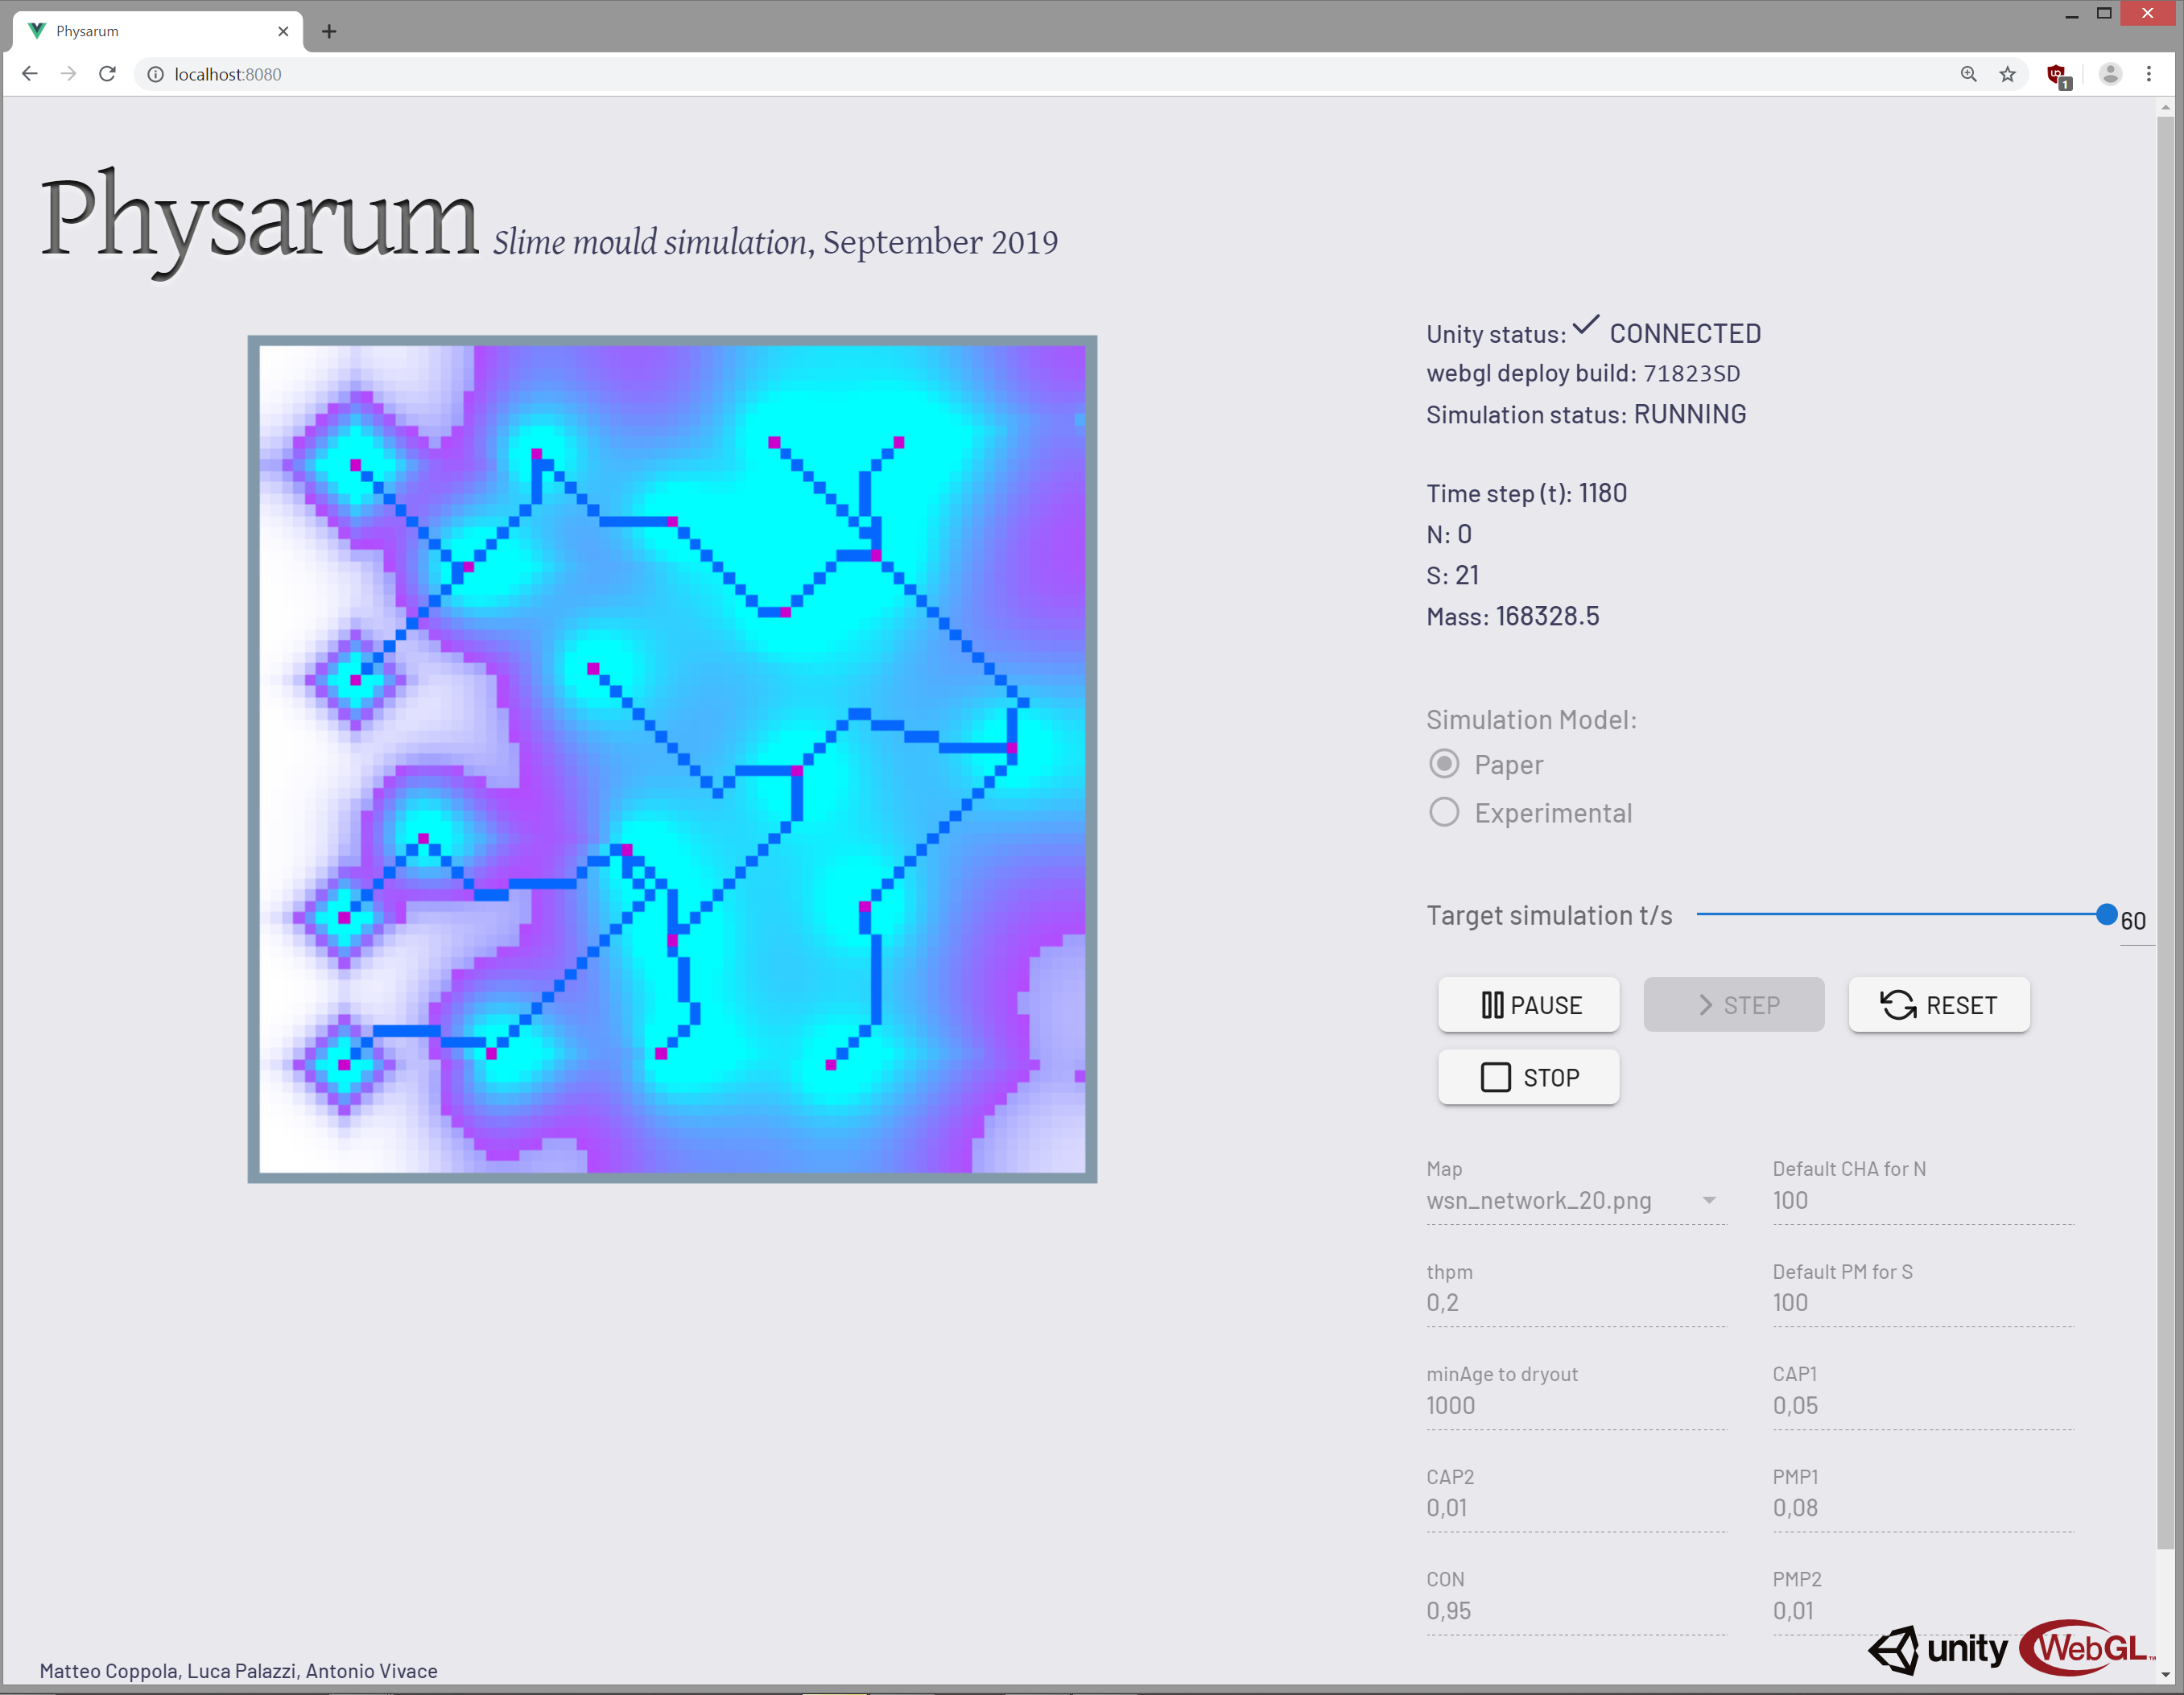
\includegraphics[width=0.8\textwidth]{UI1}%
    
  \caption{Final application view}
  \label{fig:swstack1}
\end{figure*}

\begin{figure*}
  \centering
    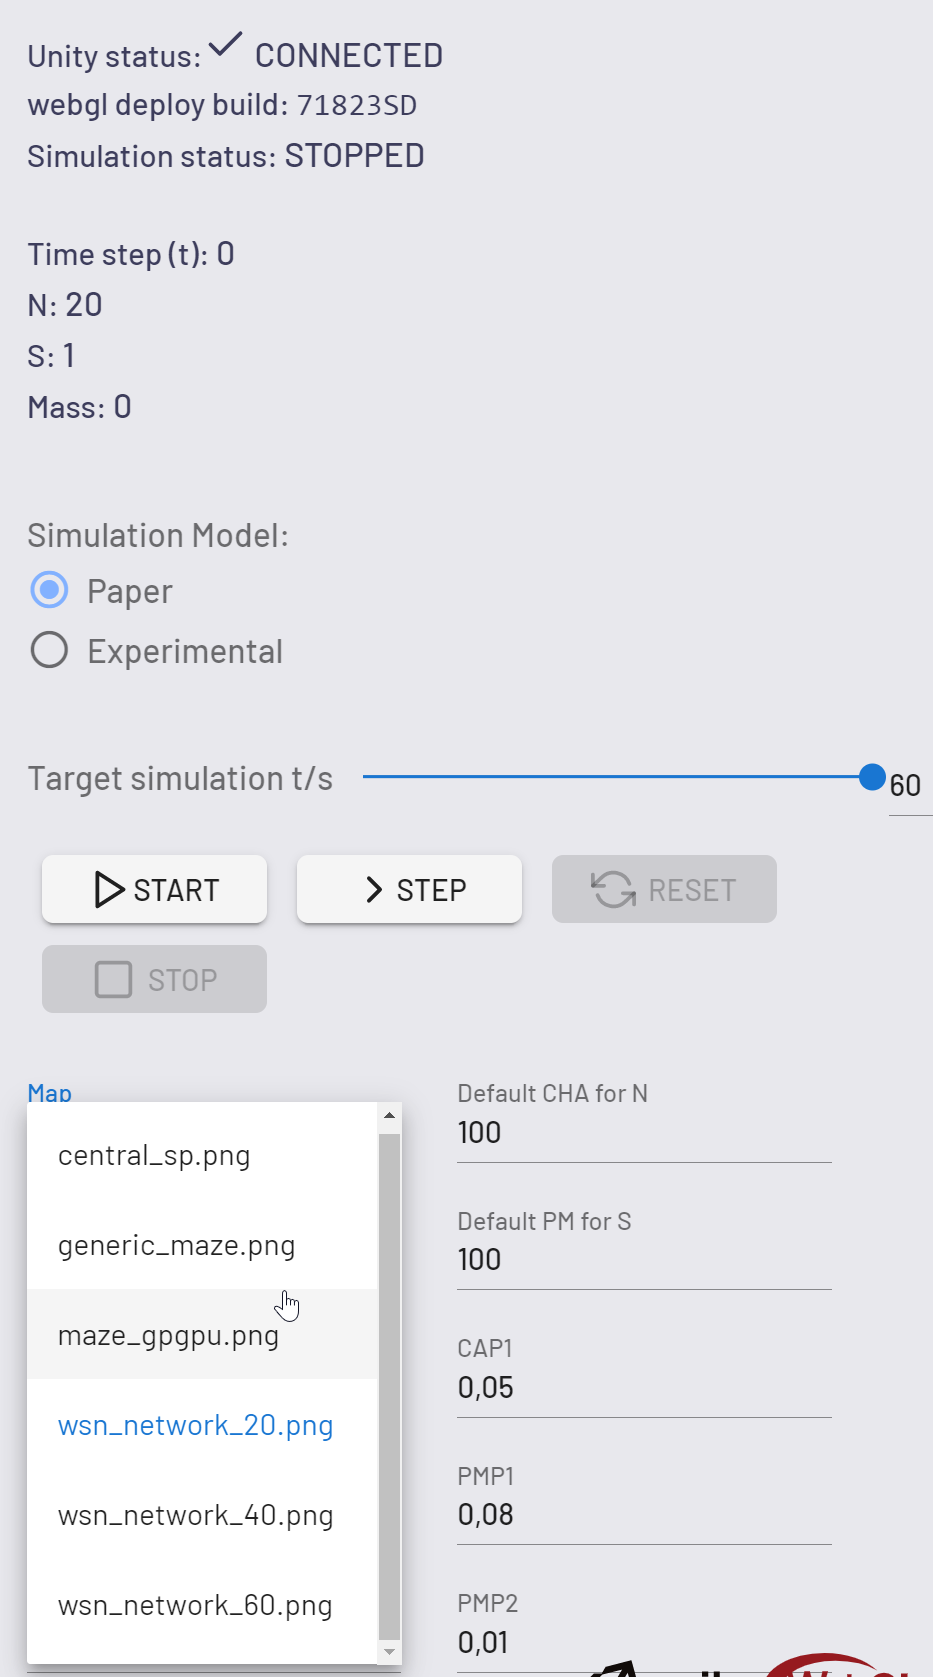
\includegraphics[width=0.4\textwidth]{UI2}%
    
  \caption{User Interface view}
  \label{fig:swstack1}
\end{figure*}

\section{Simulation framework}
\begin{figure*}
  \centering
    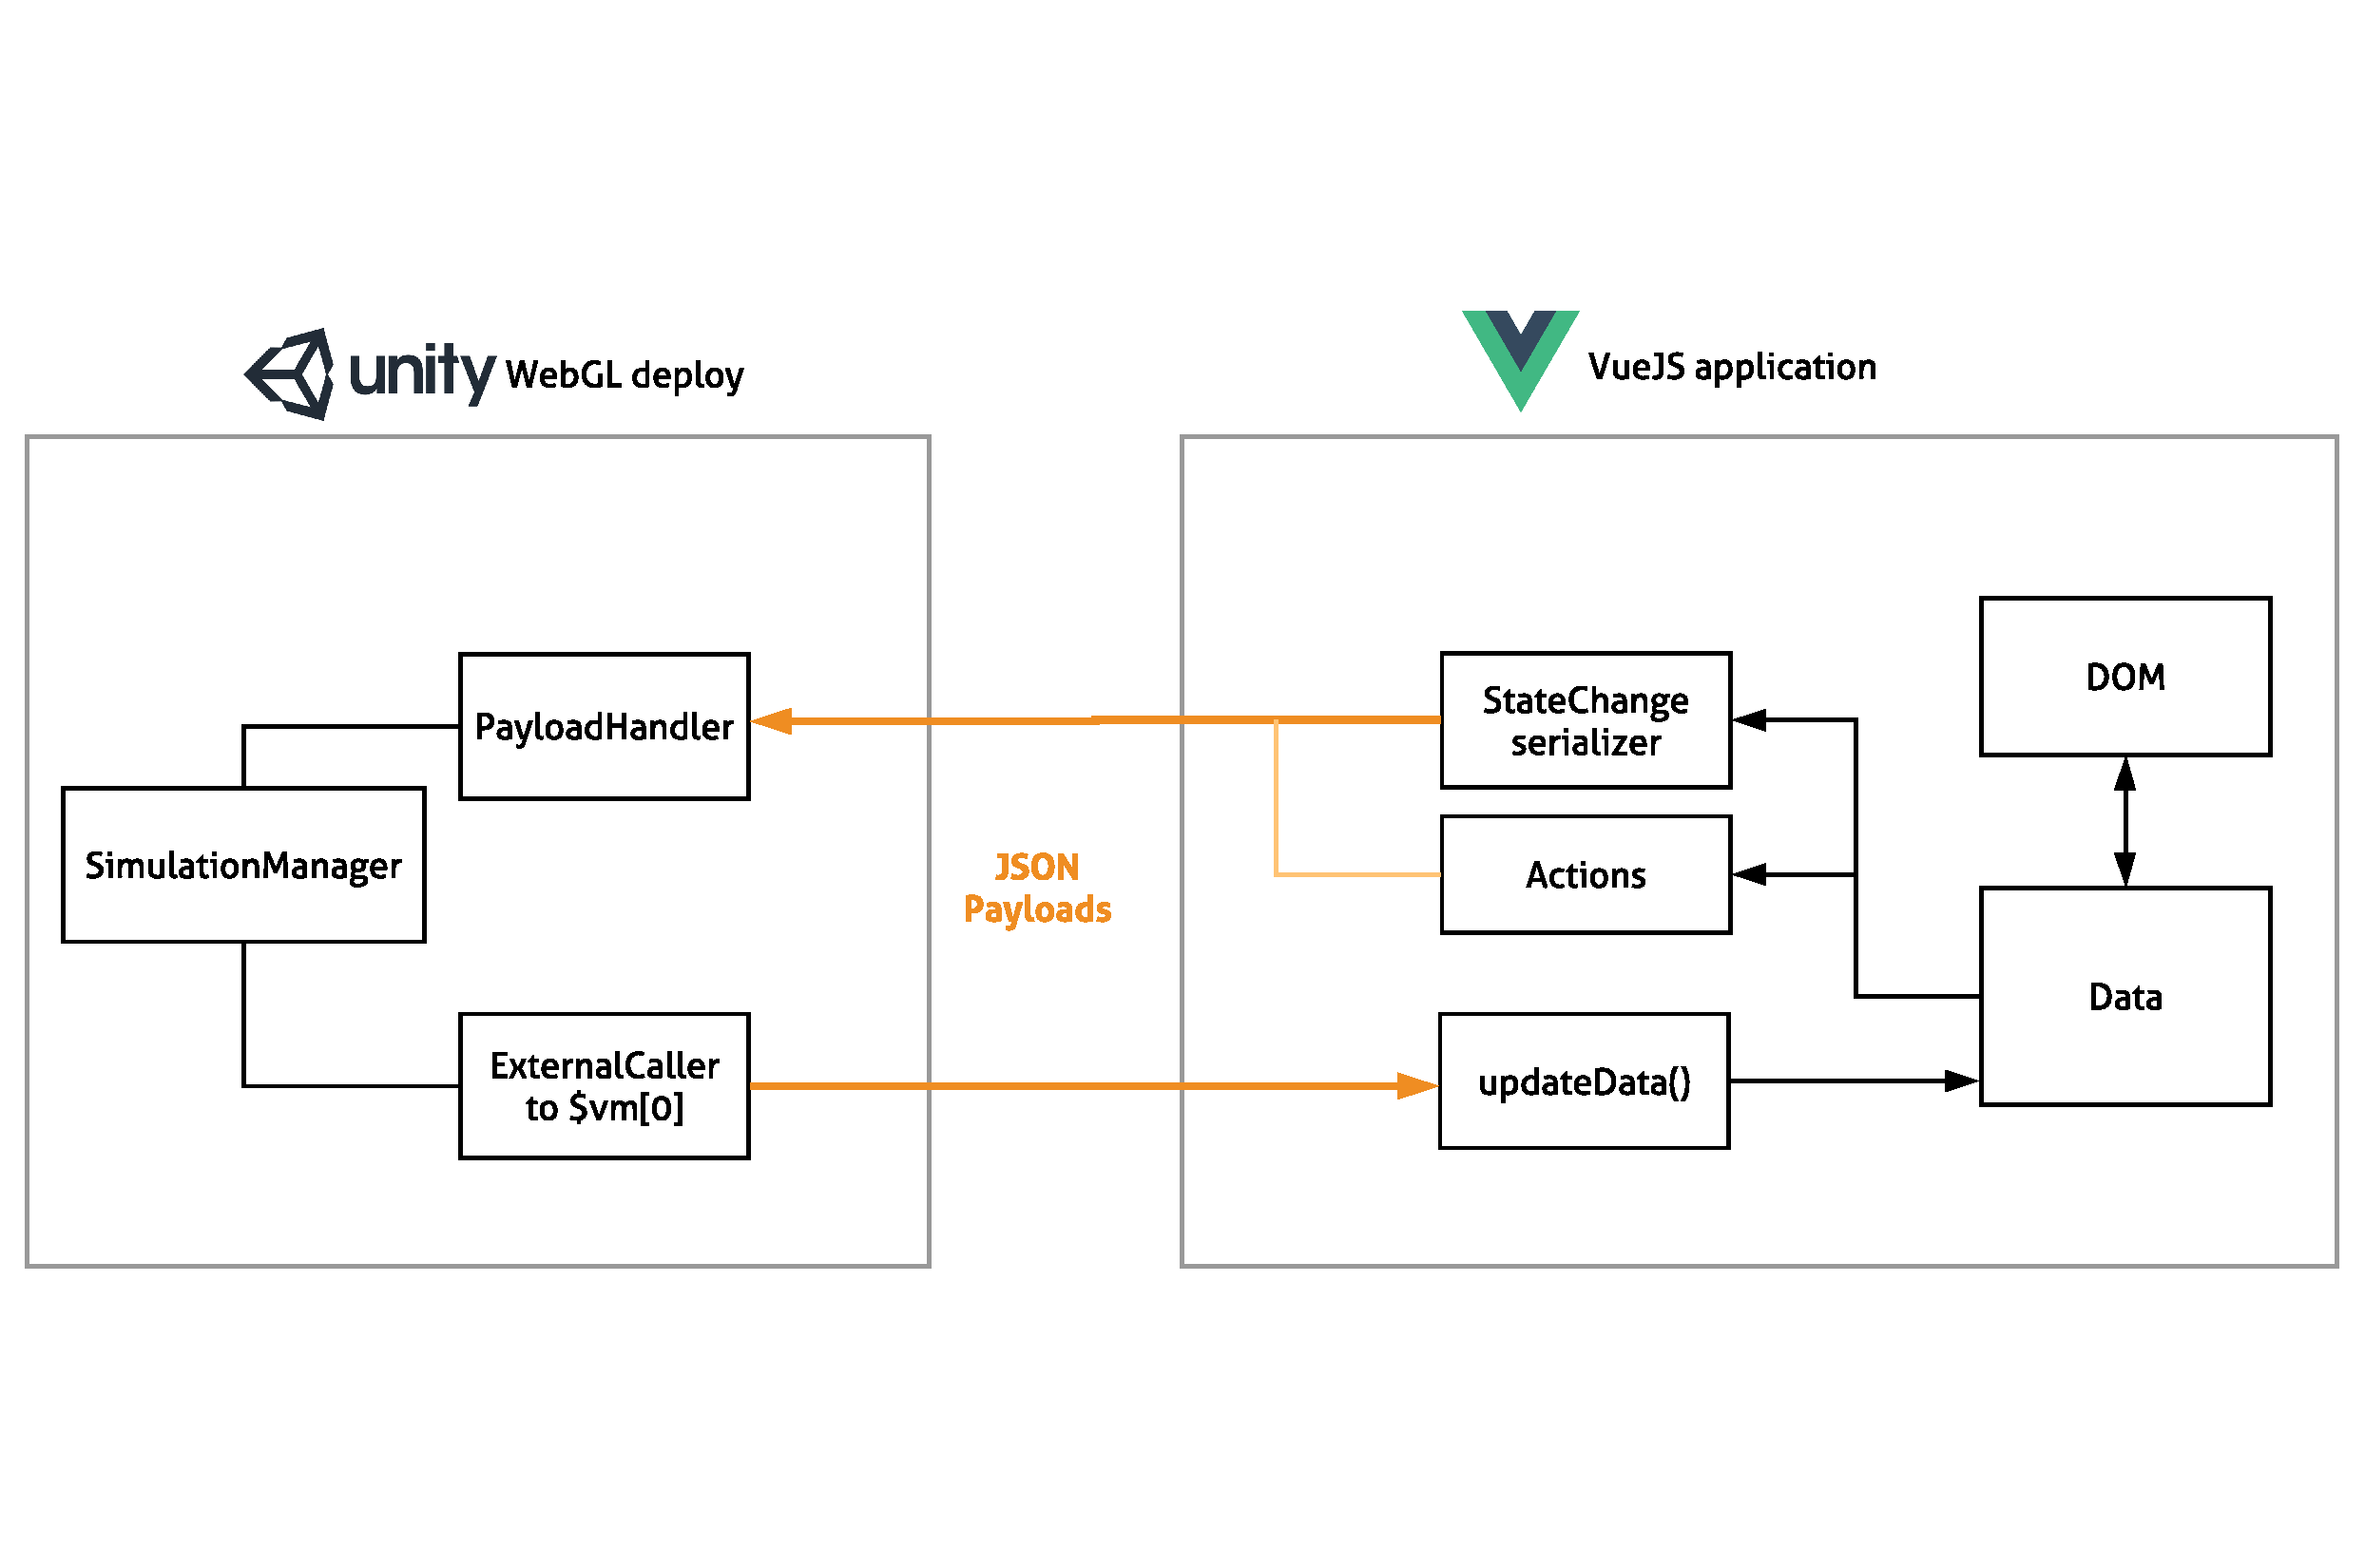
\includegraphics[width=1\textwidth]{sw_arch}%
    
  \caption{Overview of the VueJS - Unity bidirectional comunication with the Payload class}
  \label{fig:swstack1}
\end{figure*}
\subsection{Vue and Unity bidirectional communication}
After some initial experimentation, Unity emerged as suitable for the described requisites: it runs fast enough and defining local rules for the evolving values of the parameters for each cells was easy and immediate making use of a "TileMap component".

Adding Vuetify, a CSS framework providing ready UI components, to Vue.js allowed us to design a good looking and functional user interface, exposing execution control buttons, inputs and select forms to monitor and control each aspect of the simulation.

However, we needed a fast and realiable way to make those two components comunicate constantly and in both directions:

\paragraph{Vue to Unity}

When Unity is loaded, it exposes a \texttt{gameInstance} object. We can use the \texttt{SendMessage} method offered by this object to launch a public method defined inside the Unity scripts directly from the webpage embedding that Unity application. This is simple and allows passing integers and string arguments.

E.g. the following line is called by Vue whenever the \texttt{onChange} even is triggered by the FPS slider:

\begin{verbatim}
gameInstance.SendMessage("GameObject", "changeFrameRate", this.fps)
\end{verbatim}

We call the \texttt{changeFrameRate} Unity method passing the new desired framerate:

\begin{verbatim}
void changeFrameRate(int targetFps){
    Application.targetFrameRate = targetFps;
}
\end{verbatim}

\paragraph{Unity to Vue}

When the browser finishes the loading of the Vue framework, the instance becomes available as \texttt{vm.\$children[0]} and we can call any of the function exposed as "method" inside the Vue definition with this object.
In Unity, we have a \texttt{Application.ExternalCall} function which calls functionName in the web page containing the WebGL player, passing the given arguments to it. Supported argument types are the primitive types (string, int, float, string) and arrays of such types.

E.g. this is the Unity function that sends to the UI the current values of the simulation:

\begin{verbatim}
void updateParameters(){
    Application.ExternalCall("vm.$children[0].unityParamUpdate",
        defaultPMForS,
        defaultCHAForN,
        CON,
        CAP1,
        CAP2,
        ThPM,
        minAgeToDryOut,
        PMP1,
        PMP2);
}
\end{verbatim}

On Vue, this function simply acts as setter, updating its internal values with the ones provided. It's defined as follows:

\begin{verbatim}
unityParamUpdate(defaultPMForS,
    defaultCHAForN,
    CON,
    CAP1,
    CAP2,
    ThPM,
    minAgeToDryOut,
    PMP1,
    PMP2){
        this.defaultPMForS = defaultPMForS;
        this.defaultCHAForN = defaultCHAForN;
        this.CON = CON;
        this.CAP1 = CAP1;
        this.CAP2 = CAP2;
        this.ThPM = ThPM;
        this.minAgeToDryOut = minAgeToDryOut;
        this.PMP1 = PMP1;
        this.PMP2 = PMP2;
},
\end{verbatim}


Exploiting these two simple patterns, we can communicate and synchronize the two application logics. From the UI we can:

\begin{itemize}
\item Start, Stop and pause the simulation;
\item Stop and reset the simulation with the default values;
\item Run just one step at the time of the simulation;
\item Change the application target time steps/seconds;
\item Change map;
\item Change the simulation model;
\item Change the simulation parameters.
\end{itemize}

While from Unity we

\begin{itemize}
    \item Show the simulation tilemap;
    \item Send updated values about the simulation at each frame;
    \item Send the updated parameters values.
\end{itemize}

\subsection{More complex payloads}

An additional JSON serializer/deserializer class was developed even if it eventually resulted easier and clearer to just pass every parameter in a stringified array instead of building an ad-hoc Payload class with each needed property every time. 

However, this approach is much more scalable and will definitely be useful in bigger applications, e.g. when the Payload between the two components will need to carry complex and heavier (maybe binary) data such as entire custom maps.

\subsection{Developoment and deployment}

The development of the application was done on UNIX systems, using git as version control system.

Webpack is a module builder for recent web technologies, a template configuration is provided with Vue: it provides hot reload and a development server to see the application live in the browser and automatically rebuilt on each change on the Vue side.

The Unity application must be built using the WebGL target. The build artifacts must be served statically by the web application, so we can embed the UnityPlayer and the actual application alongside the VueJS instance.

GitHub, our git hosting of choice, allows to serve static webpages. We exploited this functionality to obtain an easy and fast way to continuosly deploy our application: a simple script (\texttt{npm deploy}) build the Vue.JS application for production (with the Unity webGL build artifacts as static assets), then deploys it on the "master" branch of the repository. GitHub then serves the contents of this branch with its free service GitHub Pages.

\section{Simulation lifecycle}


\paragraph{}

\subsection{Color shading}

One of the most important aspect of the simulation is how to present the results, in real time and in a meaningful and intuitive way. 

We wanted to put focus on one particular feature: the transition of the mass among cells, both on the smaller and the outer range.

This means we needed a smooth animation, making use a changing color tone, representing the steady and consistent movement and formation of the slime mould navigating the map, while expressing how the mass density was changing and moving among areas.

\paragraph{Linear interpolation approach}

The initial approach we considered was a standard linear interpolation: assuming colors are given as triples $(r_1,g_1,b_1)$ and $(r_2,g_2,b_2)$ in the RGB color system, we can fade between them with a simple \textit{linear interpolation}:

\begin{align}
r' &= (1-t)\cdot r_1+t\cdot r_2\\
g' &= (1-t)\cdot g_1+t\cdot g_2\\
b' &= (1-t)\cdot b_1+t\cdot b_2
\end{align}

This gives a blended color $(r',g',b')$ for all $t\in[0,1]$. For $t=0$ it will give the first color, for $t=1$ the second color.


$$ C_1=\begin{pmatrix}r_1\\g_1\\b_1\end{pmatrix}, \qquad C_2=\begin{pmatrix}r_2\\g_2\\b_2\end{pmatrix}$$

The blended color is given as the vector $C'(t)=(1-t)\cdot C_1+t\cdot C_2$.


\begin{figure*}
  \centering
    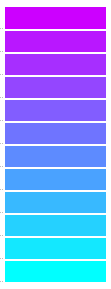
\includegraphics{colorshade1}%
    
  \caption{The chosen color shading}
  \label{fig:color}
\end{figure*}


\paragraph{Prescaling and tuning}

The value we want to represent with color is the \textit{Mass} of every single cell. This values varies greatly (and with a different rate based on the model), but we're particularly interested in the growth of smaller values (the mould exploring) and the internal movement of mass.

The different rate of growth is taken into account using two different prescale factors: the mass on the Paper model is reduced by a factor of 50, while ours is reduced by a factor of 10.

We also don't want to represent any value exceeding a threshold since nothing interesting happens after a certain value, and we do not want to focus on something not effecting the actual behaviour of the simulation. This threshold was set to 1000 for the Paper simulation and 100 for the experimental one.

\paragraph{Chosen color shading algorithm}

Following the ideas of the linear interpolation, our color shading algorithms works in the following way. We express colors in Unity's class using RGB triples, with each value in the 0-1 range.\\

PaperModel:

\begin{itemize}
    \item Empty cells are white. C= $(1,1,1)$
    \item Cell mass is scaled with a factor of 50 (40 on low-mass cells). $PM = PM/50$
    \item On low-mass cells ($PM < 15$): C= $(1-PM,1-PM,1)$
    \item C= $(1-PM,PM,3)$
\end{itemize}

Experimental Model:

\begin{itemize}
    \item Empty cells are white.
    \item Cell mass is scaled with a factor of 10. $PM = PM/10$
    \item C= $((0.8-PM)*1.25,(PM-0.20)*1.25,1)$
\end{itemize}

The result is shade of light blue to blue-purple where the lighter values represent more action, more mass and general more mass movement activity, while the darker are the expansion front of the slime mould. The color range is also confined in a precise range (light blue to purple) with offsets on the Red and Green component of the color.

\paragraph{Additional expanding shading for the Paper simulation}

Since the paper simulation is expading extremely fast with a very low amount of mass, each run launched with our color shading algorithm was immediatly flooding the entire map, making the color shading pretty much useless until the mass started to grow near the S points.

So, for the lower values, we chosen to represent the initial expansion with another color shading formula, giving a very subtle (and almost transparent) shade of blue around the front of expansion of the slime mould.